% !TEX program = xelatex
\documentclass{ctexart}
\usepackage{xcolor} % 在latex中使用颜色
\usepackage{booktabs,tabularx,multicol} % 制作表格
\usepackage{framed} % 制作文本框
\usepackage{amsmath,amsthm,amssymb,amsfonts}    % 数学符号与字体
\usepackage{hyperref}   % 添加超链接
\usepackage[left=2.0cm, right=2.0cm, top=2.5cm, bottom=2.5cm]{geometry} % 调整页边距
\usepackage{appendix}   % 附录环境
\usepackage{subfig,graphicx}    % 插入照片
\usepackage{float}      % 固定浮动体
\usepackage{lipsum,zhlipsum} %生成一些测试文本
%---------------优雅的插入MATLAB代码---------%
\usepackage{listings,matlab-prettifier} % MATLAB 美化包
\lstset{
        style=Matlab-editor,
        numbers      = left,
        numbersep    = 5pt,
        numberstyle  = \small\color{red},
        frame        = single,
        keepspaces   = true,
        tabsize      = 4,
}
%-------------标题-------------%
\title{SEIR模型}
\date{\today}
\author{xx}

%-----------做一些设置-----------%
\numberwithin{equation}{section}    % 公式标号与section的编号挂钩
\punctstyle{kaiming}    % 调整标点符号大小

%------------自定义一些命令------------%
\newcommand{\upcite}[1]{\textsuperscript{\textsuperscript{\cite{#1}}}}
\newcommand*{\dif}{\mathop{}\!\mathrm{d}}
\def\degree{{}^{\circ}}

%---------配置环境------------%
\definecolor{shadecolor}{RGB}{241,241,255}
\newcounter{problemname}
\newenvironment{problem}{\begin{shaded}\stepcounter{problemname}\par\noindent\textbf{题目\arabic{problemname}. }}{\end{shaded}\par}
\newenvironment{solution}{\par\noindent\textbf{解答. }}{\par}
\newenvironment{note}{\par\noindent\textbf{题目\arabic{problemname}的注记. }}{\par}

%-------------可控列宽的表格--------%
\newcolumntype{L}[1]{>{\raggedright\arraybackslash}p{#1}}
\newcolumntype{C}[1]{>{\centering\arraybackslash}p{#1}}
\newcolumntype{R}[1]{>{\raggedleft\arraybackslash}p{#1}}

%-----------搞个背景-------------%
\usepackage{background}
\backgroundsetup{scale=2, angle=0, opacity = 0.5,contents = {\includegraphics[width=\paperwidth, height=\paperwidth, keepaspectratio]{fig/背景.jpg}}}
%------------- 使得矩阵的最大大小超过 10 x 10-----------------%

%---------------高亮--------------%
\usepackage{soul}
\addtocounter{MaxMatrixCols}{10}
\begin{document}
\maketitle
    为了预测传染病对社会带来的影响,我们尝试建立对传染病在社会中的传播的数学模型。

    将人群分成四类:

    \begin{itemize}
        \item $S$ (Susceptible),易感者,指缺乏免疫能力健康人,与感染者接触后容易受到感染;

        \item $E$ (Exposed),暴露者,指已经被感染,处于潜伏期的人。同样具有传播病毒的能力,但不会接受治疗。
        
        \item $I$ (Infectious),患病者,指有传染性的病人,可以传播给 $S$,将其变为 $E$ 或 $I$ ;
        
        \item $R$ (Recovered),康复者,指病愈后具有免疫力的人,不可被重新变为 $S$ 、$E$ 或 $I$。
    \end{itemize}

以一天作为模型的最小时间单元,做如下假设:
\begin{itemize}
    \item $N$ 区域内总人口
    \item $r$ 每天接触的人数
    \item $\beta$ 病毒传染给健康者的概率
    \item $\gamma$ 患者康复的概率
    \item $a$ 潜伏者转化为感染者的概率
\end{itemize}
根据上述说明,我们不难得到如下常微分方程:
\begin{equation}
    \begin{aligned}
        \frac{\dif S}{\dif t}&=-\frac{r \beta I S}{N} \\
        \frac{\dif E}{\dif t}&=\frac{r \beta I S}{N}-a E \\
        \frac{\dif I}{\dif t}&=a E-\gamma \\
        \frac{\dif R}{\dif t}&=\gamma I
    \end{aligned}
\end{equation}
此方程没有解析解,我们利用龙格库塔法求解得到如下结果\ref{pic1}:
\newpage
\begin{figure}[htbp]%
    \centering
    \subfloat[$N = 10000;r = 20;\beta = 0.03;\gamma = 0.1;a = 0.1;E(0)=1$]{
        \label{pic1}
        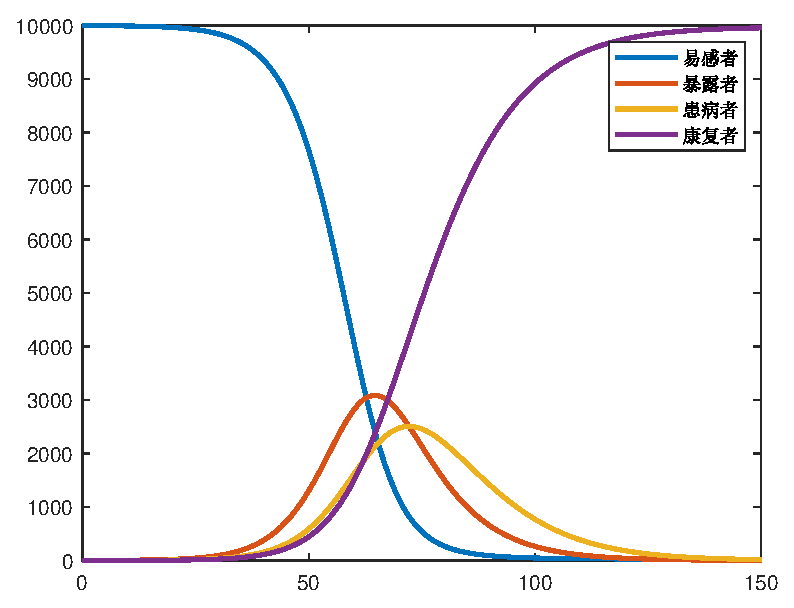
\includegraphics[width=0.45\linewidth]{fig/r=20}
        }\hfill
    \subfloat[$N = 10000;r = 10;\beta = 0.03;\gamma = 0.1;a = 0.1;E(0)=1$]{
        \label{pic2}
        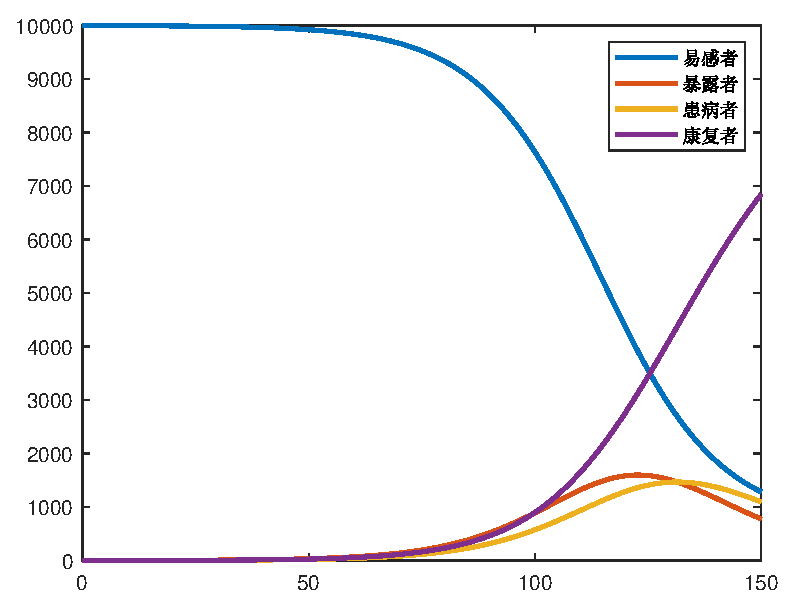
\includegraphics[width=0.45\linewidth]{fig/r=10}
        }
\end{figure}


可以看到在六十多天的时候,确诊人数达到高峰。而如果我们能减少聚集的次数,每天只和10人碰面,那么曲线如图所示\ref{pic2},这表明确诊人数的高峰被大大推迟了,假如 $r=5$,那么会得到这样的曲线\ref{pic3}:

\begin{figure}[htbp]
    \centering
    \includegraphics[width=0.5\linewidth]{fig/r=5}
    \caption{$N = 10000;r = 5;\beta = 0.03;\gamma = 0.1;a = 0.1;E(0)=1$}
    \label{pic3}
\end{figure}

在150天内,几乎没有病例的出现,曲线消失不见了。这进一步表明了我们应当服从防疫指挥,保持社交距离,减少聚集。
\clearpage
\begin{appendices}
\section{参考代码}
\lstinputlisting[title=main.m,style=Matlab-editor]{code/main.m}
\lstinputlisting[title=Runge\_Kutta,style=Matlab-editor]{code/Runge_Kutta.m}
\end{appendices}


\end{document}